Visualize a circle in MATLAB for different values of $a$, $b$, and $R$.

\begin{solution}
\begin{align*}
    0 = \left( x - a \right)^2 + \left( y - b \right)^2 - R
\end{align*}

\begin{lstlisting}
r = 1.25;
a = 0.5;
b = 0.5;
[x, y] = meshgrid(linspace(-2, 2, 200), linspace(-2, 2, 200));
f = (x - a).^2 + (y - b).^2 - r^2;
contour(x, y, f, [0, 0])
axis equal
grid on
\end{lstlisting}

\begin{center}
    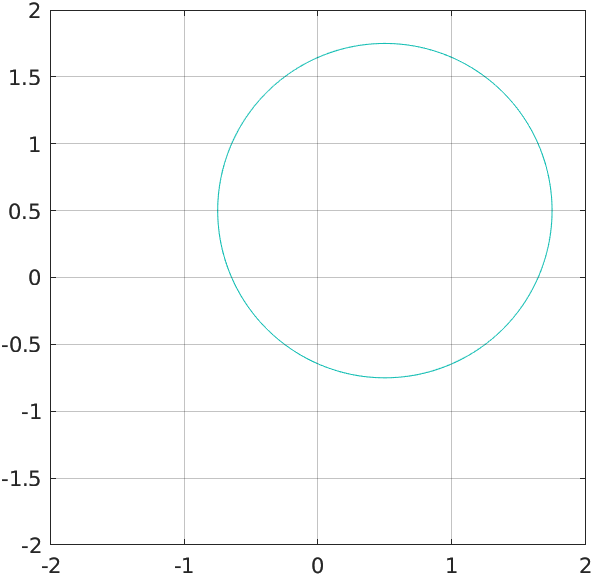
\includegraphics[width=0.5\textwidth]{img/e5p1.png}
\end{center}
\end{solution}